\documentclass[12pt]{article}

\usepackage{sbc-template}
\usepackage{graphicx,url}
    \graphicspath{{figuras/}}
\usepackage{polyglossia}
    \setdefaultlanguage{portuges}
\usepackage{microtype}
\usepackage{showframe}
\usepackage{framed}

\usepackage{subfig}
\usepackage[font=small,labelfont=bf]{caption} % Required for specifying captions to tables and figures
\usepackage{amsfonts, amsmath, amsthm, amssymb} % For math fonts, symbols and environments
\usepackage{verbatim}
\usepackage{ragged2e}
\usepackage{hyperref}
\usepackage{url}

\sloppy

\title{Identificando Idiomas com \emph{Machine Learning}}

\author{
    Jorge Ashkar Ferreira Simondi\inst{1} --- 8517081\and\\
    Leonardo de Almeida Lima Zanguetin\inst{1} --- 8531866\and\\
    Victor Luiz da Silva Mariano Pereira\inst{1} --- 8602444\\
}

\address{
    Instituto de Ciências Matemáticas e de Computação -- ICMC\\
    Universidade de São Paulo -- USP\\
    São Carlos -- SP -- Brasil
}

\begin{document}

\maketitle

\begin{resumo}
Reconhecer em qual idioma um texto está escrito, hoje em dia, é algo de suma importância. Apesar de ter várias ferramentas prontas na internet, nesse trabalho, mostraremos uma forma de como aplicar inteligência artificial para fazer essa classificação. Uma visão desde a análise dos dados até o treinamento para o aprendizado de máquina.
\end{resumo}
\section{Introdução}
\nocite{iaml:11}

\section{Análise e pré-processamento dos dados}
Para a análise do nosso problema, não seria pertinente estudar as palavras separadamente, pois não há sentido semântico. Decidimos então utilizar as letras, sem pontuação, sem espaçamento e sem dígitos.

Os caracteres especiais, como letras acentuadas, podes ser consideradas como cruciais para a predição, mas elas servem como forma de ruído, já que nomes de pessoas e de lugares podem aparecer em ambos os tipos de texto.

A quantidade de cada caractere é uma informação relevante, mas não podendo ser utilizada crua, pois se analisarmos um texto com o total de 500 caracteres em inglês que contém 50 letras “a”, não pode ser considerado em potuguês por causa da distância dele com um outro texto de 100 caracteres que comtém 50 letras “a” ser pequena. Por esses motivos, sentimos a necessidade de usar a porcentagem de ocorrência cada letra no texto.

No exemplo a seguir, temos dois textos e seus histogramas, para melhor visualisação dos dados utilizados.

\begin{framed}
    \texttt{Perceived end knowledge certainly day sweetness why cordially. Ask quick six seven offer see among. Handsome met debating sir dwelling age material. As style lived he worse dried. Offered related so visitor we private removed. Moderate do subjects to distance.\\Of friendship on inhabiting diminution discovered as. Did friendly eat breeding building few nor. Object he barton no effect played valley afford. Period so to oppose we little seeing or branch. Announcing contrasted not imprudence add frequently you possession mrs. Period saw his houses square and misery.}
\end{framed}
\captionof{figure}{Texto do Random Text Generator~\cite{site:rtg}}

\begin{framed}
    \texttt{Ainda assim, existem dúvidas a respeito de como a execução dos pontos do programa facilita a criação das direções preferenciais no sentido do progresso. Por outro lado, o novo modelo estrutural aqui preconizado cumpre um papel essencial na formulação das novas proposições.\\O empenho em analisar o consenso sobre a necessidade de qualificação exige a precisão e a definição dos relacionamentos verticais entre as hierarquias. Todas estas questões, devidamente ponderadas, levantam dúvidas sobre se a revolução dos costumes deve passar por modificações a longo prazo.}
\end{framed}
\captionof{figure}{Texto do Lero Lero~\cite{site:lero}}

\begin{center}
    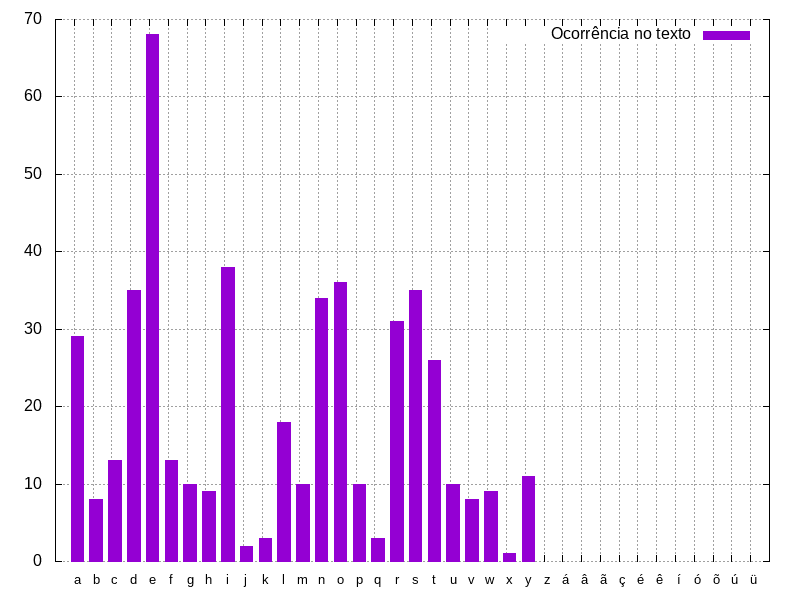
\includegraphics[width=0.8\linewidth]{freq-en.png}
    \captionof{figure}{Histograma do texto em inglês}
\end{center}

\begin{center}
    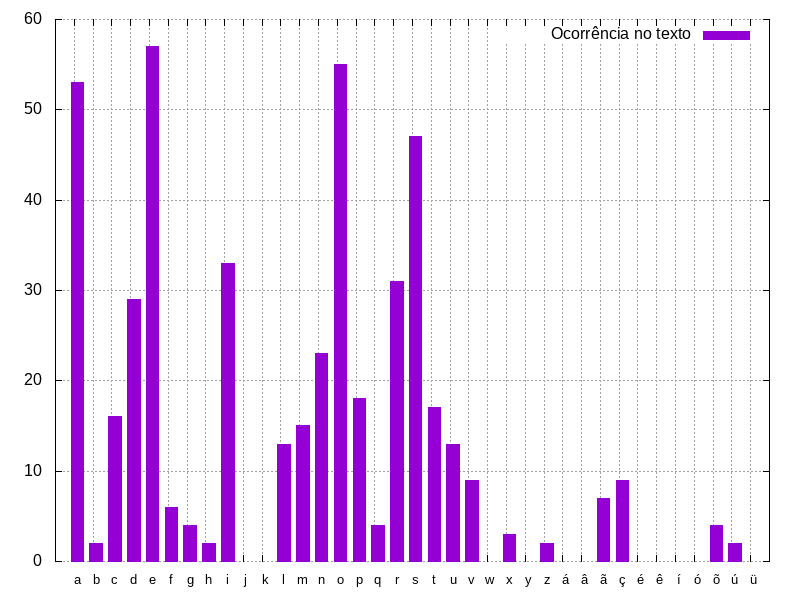
\includegraphics[width=0.8\linewidth]{freq-ptbr.png}
    \captionof{figure}{Histograma do texto em português}
\end{center}

\section{Método de classificação}
O grupo, analisando o problema, chegou a conclusão que uma solução efetiva seria usar o modelo preditivo tendo como entrada os textos da base previamente classificados e fazer uma comparação com o nosso alvo.

\subsection{Modelo baseado em distância}
A técnica que decidimos utilizar é baseado na \textbf{distância euclidiana}~(\ref{eqn:euclid}) entre o texto sem classificação e os textos da base de conhecimento. Como a distância envolvendo a quantidade de ocorrência poderia dar uma falsa informação, usamos a porcentagem que cada letra é encontrada no texto.

\begin{equation}
d(x_i, x_j) = \sqrt{\sum_{l=1}^{d} (x^l_i - x^l_j)^2}
\label{eqn:euclid}
\end{equation}

\subsection{Método \emph{k-NN}}
Para identificar em qual idioma um texto está escrito, utilizamos o algoritmo \emph{k-NN} (\emph{k-Nearest Neighbor}, em inglês). Este é um algoritmo de identificação de padrões, que consiste em verificar e comparar as frequências dos caracteres nos textos base com o novo texto, para identificar uma proximidade e decidir o idioma.

É possível melhorar o desempenho do algoritmo removendo fatores que não são de grande importância. Assim como escolher um bom valor para “\emph{k}” em cada caso reduz a chance de erro na escolha.

Como a distância para o mais próximo pode não ser tão precisa, a utilização do algoritmo \emph{k-NN}, do inglês \emph{k-Nearest Neighbor} se fez necessária, assim calculamos a distância para cada texto e fazemos uma média dos \emph{n} primeros, utilizando \(n = 3\).


\section{Resultados}
A nossa base de conhecimento se limitava a vinte arquivos bem grandes de “texto” em português e em inglês, sendo dez de cada tipo. Os textos foram gerados a partir de duas ferramentas na internet, a Gerador de Lero Lero v3~\cite{site:lero}, para textos em português, e o Random Text Generator~\cite{site:rtg}, para a produção de textos em inglês.

Com essa amostra tivemos a taxa de acerto de 100\%, o que não deixa de ser ruim, porém não pode ser considerado como um resultado relevante. Rodamos o algoritmo em cima de alguns textos fora da base de dados coletados de mensagens em redes, que também tiveram suas predições feitas com sucesso, mesmo contendo algumas formas de ruídos, como nomes próprios.
\section{Próximos passos}
O grupo pretende, para incrementar o trabalho, fazer o mesmo procedimento de classificação de idiomas utilizando uma base maior, para assim ter realmente dados concretos que o sistema está funcionando. Para essa modificação acreditamos que seja necessário aplicar a técnica de validação cruzada, a qual seleciona uma parte para ser o alvo e outra para o treino.

Como o trabalho que fizemos está baseado em duas linguas diferentes, elas diferem até mesmo a origem delas (a língua portuguesa vem do latim, já a língua inglesa surgiu nos reinos anglo-saxônicos), outro plano é fazer a predição de textos de mesma família, como o italiano e o português. Apesar de serem linguas diferentes, elas tem uma frequência de letras mais parecidas que as que usamos.


\section{Considerações finais}


\bibliographystyle{sbc}
\bibliography{sbc-template}

\end{document}
